\section{Layered Data Representation for Visual Simulation of Terrain Erosion}

%DEL: \cite{cordonnier2016large}

\begin{figure}[htb]
	\centering
	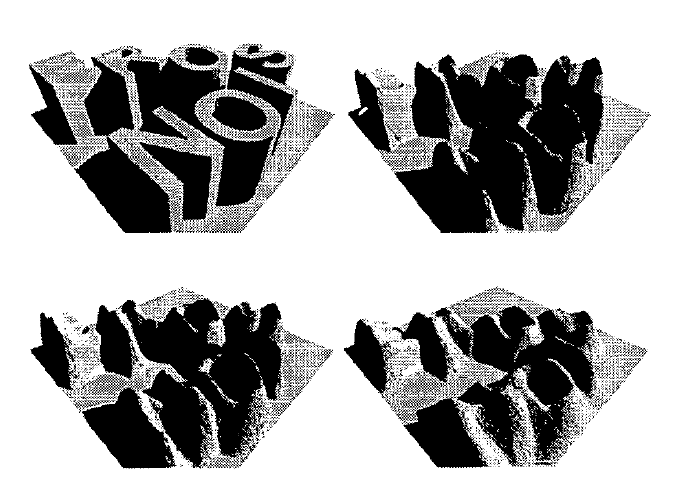
\includegraphics[width=\linewidth]{MGG_10/snap2.png}
	\caption{Thermal erosion example}
	\label{fig:thermal_erosion}
\end{figure}

This Paper \cite{marechal2010heat} focuses on introducing a completely new data-structure to store terrain-information which makes calculations much easier to perform. The two opposing conventional methods of storing and handling such data have already been explained before:
\begin{itemize}
	\item Voxel Representations which allow for accurate calculations but have very high memory demands
	\item Surface-only representations (like hight maps) of just the terrain-surface, where precision and accuracy is sacrificed in order to gain space and reduce computing time
\end{itemize}

Many different techniques have already been discussed here and many more have been developed (see Figure \ref{fig:thermal_erosion} for example). Some of the most common ones include fractal interpolation to generate hills and water streams \cite{kelley1988terrain} or blending some elaborate noise functions to generate visually plausible results (see \cite{eckbert2000simulating}, \cite{musgrave1989synthesis} and \cite{musgrave1999towards}). In this paper it is also specifically underlined, that the different attributes of present materials need to be taken into account. This might influence the erosion process quite a bit as it can be seen in Figure \ref{fig:erosiondifference}. But all of these approaches have one thing in common: while the accuracy of true 3D voxel representation is often approximated quite well, it is never truly reached with such techniques.

To overcome this limitation and allow for very accurate calculations, which are meant to be used in physical simulations rather than in real-time environments, the authors generated a mixed data-structure combining voxel and hight filed representations.

\begin{figure}[htb]
	\centering
	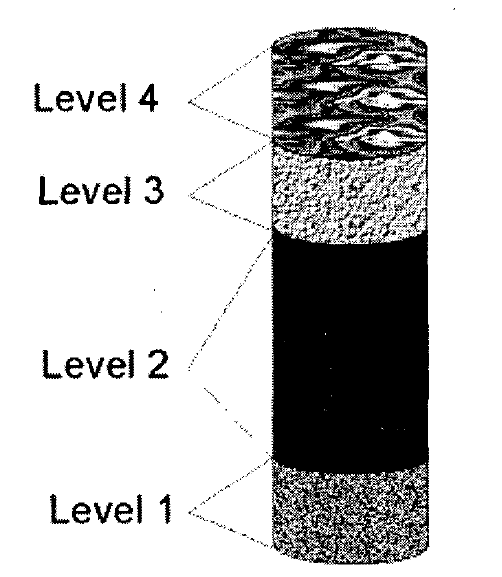
\includegraphics[width=\linewidth]{MGG_10/snap1.png}
	\caption{Layered data structure of a core sample}
	\label{fig:coresample}
\end{figure}

\subsection{A novel data structure}
Since in many areas of a given terrain are uniform and the represented layers are usually quite thick a complete set of full voxel data could be called a "waste  of data" (or rather space) \cite{marechal2010heat}. Due to that fact we can try to reduce the data to be stored in relatively uniform areas of a terrain. This approach used in this paper is to use a 2D array of 1D arrays as representation of terrain. Like illustrated in Figure \ref{fig:coresample}, it can easily be imaged as a core sample where each layer in itself is supposed to be constant (or rather its parameters are). The hight of the position can easily derived from a "core samples" hight and its index.

The big advantage of this kind of data structure is, that it's easy and fast to traversal with much smaller effort (and thus higher speed) as it would be the case for a conventional, pure voxel approach. Another positive side effect of storing data this way is that the data structure also allows zero-density layers. This way even caves and even material falling from the ceiling of those caves (along the inverted surface gradient) can be captured and therefore be used to perform calculations. That way erosion can not only be performed on the terrain-surface, but also in all sub-surface holes existing or developing in the terrain layers \cite{marechal2010heat}.

\begin{figure}[htb]
	\centering
	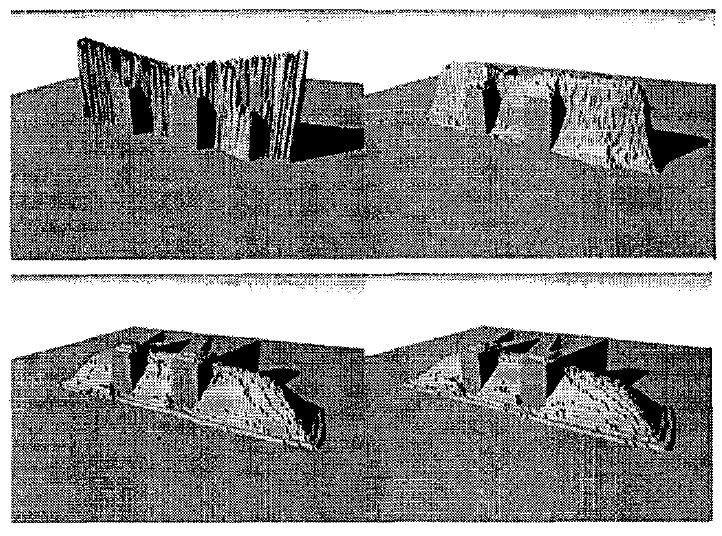
\includegraphics[width=\linewidth]{MGG_10/8582.png}
	\caption{Letter W surrounded by easily eroded material}
	\label{fig:erosiondifference}
\end{figure}

\subsection{Efficiency}
The calculations to test the efficiency of the newly introduced data structure were performed on an Intel III with 500MHz, and a freeware tool was used to generate simple visualizations. The calculation of 100 erosion steps on a 1024x1024 element grid with 5 layers took 239 minutes for example. Other calculation taking much longer were also tested, including some that could not be done with purely relying on hight filed data. The full and exact specs and results can be found in the original paper \cite{marechal2010heat}.